%%%%%%%%%%%%%%%%%%%%%%%%%%%%%%%%%%%%%%%%%%%%%%%%%%%%%%%%%%%%%%%%%%%%%%%%%%%%%%
%%
%% A sample thesis using the cssethesis class
%%
%%%%%%%%%%%%%%%%%%%%%%%%%%%%%%%%%%%%%%%%%%%%%%%%%%%%%%%%%%%%%%%%%%%%%%%%%%%%%%
%%
%% Preamble
%%

\documentclass[a4paper,11pt,bcshonoursthesis,singlespace,twoside]{cssethesis}
% * Include the option "pdflatex" above if you want to use pdflatex rather than
% standard latex to compile your document
% * Include the option "litreview" above if this is a literature review.
% * Include the option "nocoursecode" so that the numerical course code is
% suppressed after the course name.
% * Include the option "oneside" if you don't want formatting for two-sided
%   printing.
% * Include option "thesisdraft" to get a timestamp and "Draft" message in
%   the footer
% * Include option "thesispsdraft" to get a timestamp and "Draft" message in
%   the footer, along with a grey "DRAFT" in the margin. Note: this only
%   works with latex, not pdflatex

\usepackage{natbib} % Use the natbib bibliography and citation package
\bibpunct{(}{)}{;}{a}{,}{,} % use more standard Harvard punctuation
\renewcommand{\cite}{\citep} % often a useful short-cut
\usepackage{tikz} %Finite state automata
\usepackage{subfig}
\usepackage{amsmath}
\usetikzlibrary{arrows,automata}
% Definitions needed by the cssethesis class. See the documentation for
% others
\thesisauthor{Bradon Thomas Hall}
\thesisauthorlastname{Hall}
\thesisauthorpreviousdegrees{BSc, BCompSc} % Optional
%\thesisdepartment{Caulfield School of Information Technology} % Optional.
%                  Clayton School of Information Technology is the default
\thesisauthorstudentid{22051635} % Needed for litreview
\thesisauthoremail{bthal2\@@student.monash.edu.au} % Optional. Note that the @ is
											 % given as \@@. This is not
											 % necessary in normal LaTeX,
											 % but it is if you use the
											 % amsmath package - so why not
											 % get into the habit?
%\thesismonth{July} % Optional. Current month is used if this is not set
%\thesisyear{2002} % Optional. Current year is used if this is not set
\thesistitle{Simulated Evolution of Non-Regular Strategies for Repeated Games}
\thesissupervisor{Dr. Julian Garcia Gallego}
\thesissupervisoremail{julian.garcia\@@monash.edu.au} % Optional
%\thesisdedication{I luv youse all} % Optional

% start the document
\begin{document}

%%%%%%%%%%%%%%%%%%%%%%%%%%%%%%%%%%%%%%%%%%%%%%%%%%%%%%%%%%%%%%%%%%%%%%%%%%%%%%
%%
%% Front matter 
%%
\frontmatter					% start the thesis front matter.

\thesistitlepage				% Generate the title page.
\thesiscopyrightpage			% Generate the copyright page.
%\thesisdedicationpage			% Generate a dedication page (optional)
\tableofcontents				% Generate a table of contents.
\listoftables					% Generate a list of tables (optional).
\listoffigures					% Generate a list of figures (optional).

\begin{thesisabstract}			% generate the abstract page.
This is an abstract
\end{thesisabstract}                 

\thesisdeclarationpage			% generate the declaration page (optional).

%\begin{thesisacknowledgments}	% generate the acknowledgements page (optional).
%I would like to thank everyone who helped to make this possible. It has
%been an incredible journey of self-discovery, and I love every last one of
%you\ldots
%\end{thesisacknowledgments}   

%%%%%%%%%%%%%%%%%%%%%%%%%%%%%%%%%%%%%%%%%%%%%%%%%%%%%%%%%%%%%%%%%%%%%%%%%%%%%%
%%
%% Main matter 
%%
\mainmatter						% start the thesis body.

\chapter{Introduction}
Cooperation, working together for a common goal, is a widely observed behaviour. 
Many animal species, from micro-organisms to social animals, such as humans, exhibit some cooperative behaviour. 
How did this evolve, and why do exploitative variants not disrupt the behaviour? 
Study of the evolution of cooperative strategies provides insight into problems in biology or any field where competition is relevant, for example economics and the social sciences \citep{Axelrod1997}. 

How cooperation evolves in a group of individuals is not fully understood. 
Individually, exploiting cooperative behaviour gives an individual an advantage. 
But if there is no one to exploit, this strategy is not advantageous. 
Everyone cooperating gives a better outcome, but no individual has an immediate incentive to switch. 
Evolutionary Game Theory is useful for predicting the outcome of evolution where fitness of individuals is related to behaviour of other individuals of that population \citep{maynard-smith:book:1982}. 
Computational science can be used to investigate Evolutionary Game Theory, evolving populations in various simulated environments and analysing the outcome \citep{fogel1993evolving}. 

\citet{nowak:Science:2006} discussed several mechanisms for the evolution of cooperation. 
Kin selection, when cooperation with related members increases fitness of a member who shares genes. 
Direct reciprocity is another mechanism, which can be summarised as ``you scratch my back, I'll scratch yours''; this can be studied with repeated games. 
Indirect reciprocity follows, where other members of the population reward cooperators; where the choice to cooperate is influenced by the opponent's reputation. 
Nowak also discusses Network Reciprocity, where networks of cooperating members forms. 
Finally, group selection, where success of groups of individuals and success of individuals themselves is important. 
Several of these examples (particularly kin and group selection) are various forms of population structure, which will be studied in the project. 

This project aims to investigate the evolution of cooperation in repeated games, and how the computational capability of agents in the model effects the evolution of cooperation. 
A repeated version of a simple game called the Prisoner's Dilemma will be used to simulate evolution in a competitive environment with a population of players. 
The strategies players use are randomly mutated (a Genetic Programming method), and ones that perform well in the game selected for survival- this is inspired by biologic evolution. 
This technique has been widely used to investigate behavioural biology with game theory, but richer models are necessary to improve applicability \citep{McNamara2013}. 
This work intends to contribute towards that goal. 

Strategies in repeated games can be studied via a variety of means; analytic evaluation of strategies from game theoretic approaches is one method. 
This method is particularly powerful for the study of simple strategies, or small sets of strategies. 
Computational methods provide a means to study a wider variety of strategies \citep{fogel1993evolving}. 
Using a representation that allows strategies to be mutated by a simple stochastic process allows the simulation to explore a set of strategies without manual input. 
For example, in a Finite State Automata implementation states and state transitions can be added and removed to form a new strategy. 
Strategies are removed from the population as a result of the outcome of the repeated game- the fitness of the strategy determines its survival. 
The results of simulations can be used to inform analysis of the these strategies, and analysis of how these strategies evolve.

Cooperation in repeated games was investigated by \citet{van-veelen:PNAS:2012}. 
They looked into two models of cooperation- direct reciprocity and population structure- and the relation between them, using Finite State Automata to represent strategies in the simulation. 
In this project more computationally powerful methods of representing strategies will be tested and the results compared to previous research.

The results may assist in general by further revealing the limitations or usefulness of simple evolutionary models. 
In particular, recent research has provided models with cooperation resembling human behavior more closely, and this project may help to refine, extend, or find limitations of this model.

\section{Research Context}
\subsection{The Prisoner's Dilemma}
The Prisoner's Dilemma is a simple model that has been widely used to study cooperation in repeated games \citep{Axelrod1997}. 
In the one-shot version of the Prisoner's Dilemma, cooperation is not the expected outcome. 
In this game, two players play a single game, choosing between two options; cooperate or defect. 
Players choose simultaneously, and have no information on the opponents choice before their own decision is made. 
If they both cooperate they receive a score of R (Reward for cooperation). 
If they both defect, they receive a score of P (Punishment for defection). 
If one player defects, and their opponent cooperates, the defector is rewarded with T (Temptation to defect). 
If a player cooperates, and their opponent defects, the cooperator receives a payoff of S (Sucker's punishment). 
The hierarchy of payoffs goes $T>R>P>S$. Table \ref{table:payoffs} shows the payoff matrix for the Prisoner's Dilemma. 
\begin{table}[h]\centering
\captionsetup{justification=centering}
\begin{tabular}{|l|c|c|}
\hline
 & Cooperate & Defect\\
\hline
Cooperate & R & S\\
\hline
Defect & T  & P \\
\hline
\end{tabular}
\caption{Payoff Matrix for the Prisoner's Dilemma.\\ Player choice left, opponent choice top.}
\label{table:payoffs}
\end{table}

Assuming both players are aware of the payoff table and both players act to maximise their personal payoff, defection is the strategy both players choose. 
If the opponent defects, the best move is to defect too to avoid paying the cost. 
If the opponent cooperates, the best move is to defect to avoid the cost, and gain the benefit. 
That is, the player can only lessen the payoff by cooperating- this is a Nash equilibrium. 
The dilemma arises from the fact that mutual cooperation would be a better result for both players than the equilibrium of mutual defection. 
This game captures the essence of the problem of cooperation. %Couldnt improve on JGs wording
%\pagebreak[4]
\subsection{Assortment}
In order for cooperative behaviour to compete successfully with non-cooperative behaviour, some advantage needs to exist. 
The evolution of cooperative behaviour from a population of randomly interacting members is problematic \citep{axelrod:Science:1981}. 

A solution in order to allow evolution of cooperative behaviour is to add structure to the population. 
This also better reflects most situations that can be modelled with evolutionary simulations \citep{eshel:PNAS:1982}. 
In nature, interaction between members of a population is not likely to be randomly distributed; interaction is more likely between kin, or social peers. 
Structure can be added by changing the probability of interactions- a subset of a population is more likely to interact with that subset. 

The expected payoff for a strategy in both a structured and unstructured environment can be found analytically \citep{van-veelen:PNAS:2012}. 
Consider a strategy space consisting of only always defect and always cooperate (ALLD, ALLC). 
The potential payoff ($\Pi$) for each strategy can be calculated by the probability of meeting an ALLC opponent times the payoff in that instance plus the probability of meeting an ALLD opponent times the payoff in that instance. Where $N_{TYPE}$ is the number of a type in a population, and $N_{TOTAL}$ is the total population size ($N_{TOTAL}=N_{ALLC}+ N_{ALLD}$), the payoffs are:
\begin{align*}
\Pi_{ALLC}&=\frac{N_{ALLC}-1}{N_{TOTAL}-1} \cdot (R) + \frac{N_{ALLD}}{N_{TOTAL}-1}\cdot ({S})\\
\Pi_{ALLD}&=\frac{N_{ALLC}}{N_{TOTAL}-1} \cdot (T) + \frac{N_{ALLD}-1}{N_{TOTAL}-1}\cdot ({P})
\end{align*}

In the case of an unstructured population, since $T>R$ and $P>S$, $\Pi_D$ always has a better payoff (excluding the case when $N_{ALLD}=0$). 
Instead take the case when the population is structured, and chance of meeting an alike player is r (structure parameter):
\begin{align*}
\Pi^{(r)}_{ALLC}&=(1-r)\Pi_{ALLC}+ rR\\
\Pi^{(r)}_{ALLD}&=(1-r)\Pi_{ALLD}+ rP
\end{align*}

Sufficiently higher probability of meeting an alike player allows cooperativity to have the greater payoff. 
Trivially, if probability of meeting like is 1, $\Pi^{(S)}_{ALLC}=R>\Pi^{(S)}_{ALLD}=P$, so cooperation has higher fitness.  
Substitution of values shows it holds for other cases. 
For example, if T=3, R=2, P=1, S=0, and the population is 50 ALLC and 50 ALLD:
\begin{align*}
\Pi^{(S)}_{ALLC}&=(1-r)(2\frac{49}{99})+r*2=\frac{98}{99}+\frac{198}{99}r-\frac{98}{99}r=\frac{1}{99}(98+100r)\\
\Pi^{(S)}_{ALLD}&=(1-r)(3*\frac{50}{99} + \frac{49}{99})+ r*1=\frac{199}{99}-\frac{199}{99}r+\frac{99}{99}r=\frac{1}{99}(199-100r)
\end{align*}
So ALLC has higher fitness if $r>101/200$. These cases demonstrate that structure can benefit cooperation. 
Next, repetition of games needs to be accounted for. 
%\pagebreak[4]
\subsection{Direct Reciprocity}
When the Prisoner's Dilemma is played multiple times, all parties defecting is no longer the only successful strategy, even without structure. 
For the repeated Prisoner's Dilemma, the number of games played is not known by players in advance. 
If both players knew how many rounds were to be played, the best move in the last round is defection. 
The same logic causes the second last round to be a defection, and the problem reduces to the Nash equilibrium of the one-shot version. 
A way to accomplish having an unknown number of rounds is to make future encounters probabilistic, the chance of another encounter between two players is the continuation probability $\delta$.

\citet{garcia:PLoSOne:2012} calculate the payoff for strategy A from repeated games with strategy B as
\begin{equation}
\label{eqn:repeatedPayoff}
\Pi_{AB}=(1-\delta)\sum^{\infty}_{t=0} \delta^i\pi^i_{AB}
\end{equation}
where $\delta$ is the continuation probability, and $\pi^i$ is the payoff from the $i$th round. 
The sum represents the diminishing likelihood of another game between the two players. 
The term $(1-\delta)$ is for convenience, normalising the payoffs.
 
Two simple strategies possible in the repeated version are Tit-For-Tat (TFT) and Suspicious Tit-For-Tat (STFT). 
Tit-For-Tat starts cooperating on the first round, then reciprocates the opponents last move. 
Suspicious Tit-For-Tat defects on the first round, then reciprocates the opponents last move. 
If ALLC plays TFT, in all rounds they are cooperative.  
If TFT plays STFT they alternate defect and cooperate (Figure \ref{table:reciprocity}). 
This behaviour is an example from another model for the evolution of cooperation; direct reciprocity. 

\begin{figure}[h]
\centering
\captionsetup{justification=centering}
\begin{tabular}{|l|c|c|c|c|}
\hline
TFT & C & D & D&...\\
\hline
ALLD & D & D &D&...\\
\hline
\end{tabular}\hfill
\begin{tabular}{|l|c|c|c|c|c|}
\hline
TFT & C & D&C&...\\
\hline
STFT & D & C&D&...\\
\hline
\end{tabular}\hfill
\begin{tabular}{|l|c|c|c|c|c|}
\hline
ALLC & C & C&C&...\\
\hline
STFT & D & C&C&...\\
\hline
\end{tabular}\hfill
\caption{Simple strategies playing the Prisoner's Dilemma, including reciprocating strategies TFT and STFT }
\label{table:reciprocity}
\end{figure}

The previous combination of strategies can be examined analytically. 
Equation \ref{eqn:repeatedPayoff} indicates a natural representation for the payoff of strategies as a matrix. 
Comparisons can then be made between strategies, as done above but quantitatively. 
Further, it can be determined what strategies will be selected for \citep{imhof:PNAS:2005}. 
For example, a small number of ALLD can quickly dominate ALLC since ALLD gains a better payoff. 

\subsection{Strategy Representations}
Strategies for repeated games can be represented by a variety of methods. The choice of representation has important implications. 
For example, consider a representation that consists of a binary string of length 3 \citep{garcia:PLoSOne:2012}. 
The first digit represents the move performed in the initial game, when no history exists between two players. 
A $0$ represents a choice to cooperate, a $1$ represents a choice to defect. 
The next two digits determine the choice made, based on the previous choice made by the opponent and ignoring all previous history. 
The second digit in the three digit string describes what the strategy does in response to a cooperation. 
The final digit describes what the strategy does in response to a defection. 
Table \ref{table:binaryStrategy} describes some of the possible strategies.

\begin{table}[h]
\centering
\captionsetup{justification=centering}
\begin{tabular}{|l|c|c|}
\hline
 Strategy & Description & Representation\\
\hline
ALLD & Always Defect & 111\\
\hline
ALLC & Always Cooperate & 000\\
\hline
TFT & Cooperate, then repeat opponents last move & 001\\
\hline
STFT & Defect, then repeat opponents last move & 101\\
\hline
\end{tabular}
\caption{Binary String representation for strategies}
\label{table:binaryStrategy}
\end{table}

The length 3 binary string method can explore a set of $2^3=8$ strategies. Increasing the size of the string can allow consideration of larger sets of history. 
Finite State Automata (Figure \ref{fig:fsa}) can be used to represent the same set of strategies, plus an infinite number more (not the set of all strategies however).
****FIGURE OF STRATEGY****

The strategy space (set of strategies) representable by a method is not the only important factor. 
The distance in strategy space between strategies can be defined as the number of mutations needed to turn one strategy into another. 
A possible mutation method for the binary string would be to flip a digit. 
In the case off ALLD and STFT, the distance is one. Flipping the second digit turns one into the other. 
The distance between the Finite State Automata representations is larger. 
The actual distance will depend on how mutations are performed. 
A state needs to be added to turn ALLD into STFT, 2 transitions added, and 1 transition moved (Figure \ref{fig:fsa}). 
To turn STFT into ALLD, a specific node is removed- the cooperate node- 2 transitions are removed, and 1 transition is moved. 
The implication of this example is that the 'topology' of the strategy space depends on representation. 
The path for evolution of a strategy differs based on this topology. 
If mutations are single flips on a string, the strategies exist on the corners of an n-dimensional hypercube where n is the length of the string. 
Adding another mechanism, such as flip all bits, changes the topology since opposite corners now have a new path to each other of length one.

Another example of this differing topology is the conversion of ALLD to ALLC and vice versa. 
In this example the mutation method for the Finite State Automaton is obvious; the outcome of the single node is flipped. 
The distance between strategies is one node flip. 
If the mutation method for the binary representation is to flip a bit, that is the flipping of all bits at once is excluded as a method, the distance in this strategy space is 3. 
Representation and mutation method both have important implications.

The history of moves consists of a sequence of options, cooperate (C) or defect (D). 
A strategy can be considered a formal language. 
Cooperation occurs when the history belongs to the language. 
Figure \ref{fig:fsa.lang} shows the Finite State Automata approach to this. 
Finite State Automata, the representation used in \citet{van-veelen:PNAS:2012}, allows only regular languages, which restricts the strategy space. 
To make the problem tractable, some representation that only represents a subset of possible strategies is required. 
Each representation for strategies has limitations, advantages and disadvantages, such as the set of strategies that can be simulated and complexity of mutation. 
In this project, non-regular strategies will be simulated.

The methodology from \citet{van-veelen:PNAS:2012} will be followed with this new representation, and how non-regular strategies effect the results examined.

****FIGURE****
\section{Research Plan and Methods}
\subsection{Selecting Representations}
Adding computational power to agents could be accomplished by using Deterministic Push-Down Automata (DPDA), allowing the exploration of a strategy space including all strategies representable by Deterministic Context-Free Languages. 
Whilst I cannot predict what strategies will evolve, I can give examples of what strategies could evolve that could not in a regular strategy space. 
One example is making a decision based not on the exact sequence of moves, but on the ratio of moves. 
A pushdown automaton can check if the opponent has been overwhelmingly uncooperative (say, defecting 3/4 of the time) and pursue a different strategy based on this assessment. 
Since regular languages are a subset of Deterministic Context-Free Languages \citep{Sipser2006}, a pushdown automata can represent all strategies used in \citet{van-veelen:PNAS:2012}. 

The DPDA is by no means the only representation that could be selected, but highlights the task the of selecting a representation. 
More computationally powerful methods could also be used. 
These would have associated advantages like allowing a larger strategy space. 
Disadvantages include the possibility of infinite loops developing in strategies.

In this project, selecting a representation to use is the first task that must be completed. 
This will be performed in conjunction with the literature review; previous approaches to this problem in the literature will inform the decision. 
The decision process will also include prototyping each representation and examining the feasibility of using it in simulations.
%\pagebreak[1]
\subsection{Simulation}
A simulation will be created in Java, using an agent based model, based on \citet{van-veelen:PNAS:2012}. 
Test driven development methodology will be used, using JUNIT for unit tests. 
The simulation will consist of representations for strategies, a Wright-Fisher mutation process for representations, a Prisoner's Dilemma game and a selection process based on performance in the Prisoner's Dilemma. External libraries will be evaluated early in the design of the the simulation for possible use. 
Factors such as extensibility for further research such as using a different mutation process, representation or basis for structure will be considered. 

A process of stochastic mutation and selection will evolve strategies. 
To investigate the relation between structure, direct reciprocity and cooperation, assortment of the population and continuation probability will be variable. 
Simulations will be designed with best practices for scientific computing in mind \citep{wilson2014best}. 
For analysis, information such as strategies that appear in the simulation, their frequency and how long they remain in the population will be recorded. %Not reproducibility of research, thats a different thing
%\pagebreak[1]
\subsection{Analysis}
The results of the simulation will be examined, discovering the variety of strategies that evolve. 
Evolution paths, mechanisms by which strategies become a fixture in the population (such as direct invasion and indirect invasion), and cycles in the simulation between dominant strategies may be examined. 
This includes patterns such as strategies invading another strategy directly (beating it directly) and indirectly (becoming fitter than a strategy by performing better against the general population). 
For example indirect invasions display interesting cycles, where the invader does not excel until an exploitable strategy becomes sufficiently frequent in the population \citep{van-veelen:PNAS:2012}. 

This will involve some work using game theory to analyse strategies, as well as analysis of the results of the simulation. 
In particular the relation between the structure of the population, the reciprocity of the population, and the resulting cooperativity will be examined. 
%\pagebreak[4]
\section{Deliverables}
In this project an agent based simulation of evolution useful for exploring the relation between reciprocity and population structure will be produced. 
The simulation will extend the work of \citet{van-veelen:PNAS:2012}, using more computationally powerful representations for strategies. 
Software produced will consist of a simulation written in Java, unit tests for all aspects of the simulation, and technical documentation. 
It is intended the source code for this simulation will be made publicly available at the end of the project, and be part of the scientific contribution for this project. 
An analysis of the results of this simulation in the context of conclusions from previous research and game theory will also be completed. 
\chapter{Literature Review Chapters}

\section{Direct Reciprocity}
\label{sec:dr}
Direct Reciprocity has been widely studied, with both analysis using game theory and simulations. 
When the game is repeated, the possible strategies are no longer simply Cooperate or Defect. 
Now, the players choose what to do over a series of games. 
In the repeated Prisoner's Dilemma, infinite strategies exist.

If the game is repeated a fixed number of times, no cooperation is expected- if all possible strategies are permitted. If both players know the number of rounds to be played, the result of the one-shot Prisoner's Dilemma is expected during the last round: mutual defection. Backward induction leads to a fully defecting game \citep{aumann1995backward}. This can be avoided by having probabilistic length games. 
Instead of playing a fixed number of times, strategies play each other once, then with probability $\delta$ they play again, resulting in a probabilistically determined game length. 

Playing the Dilemma results in a payoff/fitness which is used to determine both how a player performed, and to select players to reproduce or survive. All payoffs are positive (to avoid negative fitness), so if payoffs from each individual game were simply summed, there would have been an advantage to playing more rounds. To account for this, the rounds can be summed with a discount weight:

\begin{equation}
\Pi_{AB}=(1-\delta)\sum^{N}_{i=0}{\delta^i\pi^i_{AB}}
\end{equation}
Where $\Pi$ gives fitness after a sequence of games, and $\pi^i_{AB}$ is the payoff A recieves playing B in the ith game between them.

\subsection{Axelrod's Tournaments}
\citet{axelrod:Science:1981} investigated the behaviour of strategies using computer tournaments, with repeated Prisoner's Dilemma games played between strategies submitted by people to the tournaments. 
This study compared fitness (payoff of games) of submitted strategies playing each other. 
Strategies play each other probabilistically; the game is not a fixed size, instead a continuation probability determines if they continue to play. Out of the 14 submitted strategies, Tit-For-Tat (TFT) performed best. 
This is a simple strategy that reciprocates the other player's behaviour, after initially cooperating. 
Initially it cooperates, then it repeats the other player's last move. 
When playing a strategy that always cooperates (ALLC), it performs identical to ALLC. 
When playing a strategy that always defects (ALLD), it loses on the first turn, then performs identical to ALLD- given a long enough number of games played, the strategies have similar payoffs. 

Axelrod and Hamilton identified three criteria to determine if a strategy can be successful. The strategy must be robust- it must perform fairly well against a wide variety of strategies. TFT does so, including against the a population composed of the simple ALL* examples, but only if there is a sufficient chance of the game repeating. Secondly, the strategy must be stable- a mutant strategy must not be able to invade in the event the strategy becomes established. For example, ALLC is not stable against ALLD. 
A single ALLD in a population of ALLC will gain better payoffs (fitness) and invade. 
Lastly, the strategy must be initially viable- it must be able to gain a foothold. 

The Tournaments provide insight into the role Direct Reciprocity can play as a mechanism for the success of cooperation. 
A desirable extension is to allow evolution of the strategies, rather than just allowing the example strategies to compete. 
From the outcome of the tournaments one might initially suspect Tit-For-Tat might emerge and always dominate. However, \citet{boyd1987no} showed this might not be the case; Tit-For-Tat is not (and indeed no strategy is) evolutionary stable in the repeated dilemma game \citep{boyd1987no, van2010and}. 
%Axelrod also let the players compete in an evolutionary environment. 
%*Axelrod population vs population 1987 might be worth it here*

\subsection{Evolving Strategies in Simulations}
\label{sec:axelrodEvolving}
\citet{axelrod1987evolution} used a simple Genetic Algorithm approach to study the evolution of strategies for the Prisoner's Dilemma \citep{back1997handbook}. A half-memory approach is one in which the opponent's sequence of Cooperate (C) or Defect (D) moves are remembered. A full memory approach remembers its own moves, or equivalently the results (both C is the same as Reward, R, both D is the same as Punish, P, etc). A string of \{C,D\} represents each strategy. A Full-Memory approach was used in \citet{axelrod1987evolution}. 

Based on previous moves, a location in that string is looked up, and states the next move to perform. 
The first 6 bits determines the initial strategy, then there is not a history of 3 moves. 
It gives a `history' to base decisions on, when no actual history is available. 
6 bits are required since both the opponents and their own moves need to be encoded. 
To encode the strategy, 64 bits are used. Three moves are remembered, with 4 possibilities- so $4^3$. 
A total of 70 bits were used by Axelrod's simulation, allowing for moves to be determined based on the last 3 results. That is, it is a full-memory simulation of length 3. 
This allows for any of $2^{70}$ different strategies to appear- analysis using a matrix of payoff of every strategy against every other strategy would be a square matrix with $2^{70}$ elements on each side. 
This is why explicit analysis selects notable examples from the population, and demonstrates why simulation will be useful. 

Strategies were evolved using Genetic Algorithms. Strategies are generated in a population, and then they compete with 8 strategies from the original tournaments to determine their fitness. A new population is determined by reproducing from the population, with fitness determining what strategies reproduce. They then compete with the 8 representatives again. 
Reproduction involves a small chance of random mutation, and a crossover from each parent. 
The string representing the strategy is the chromosome, and the new child is produced from parts of each parent's chromosome. A population of 20 strategies competed in games 151 moves long, competing with 8 other members of the population in each round, for 50 generations. 
Technology of the time limited the size of simulations; today we have the luxury of being able to throw far more computing power at the problem, allowing for much longer (and with larger population) simulations. 
The initial population was random. The strategies that evolved mostly resembled Tit-For-Tat, and Axelrod identified general patterns for strategies. They continued cooperating after mutual cooperation had been established, they responded to opponent defection with defection, they returned to cooperation after it was restored by the opponent following a defection, and when stuck in a pattern of mutual defection they do not attempt to escape and allow themselves to be exploited. 

Strategies that performed better than Tit-For-Tat did emerge. These developed ways to exploit one of the 8 representatives, having a higher fitness against that, at a cost of a lower fitness against some of the other 8 representatives. If the net result is a gain over Tit-For-Tat, the strategy performs better. 
This only applies to the environment of this simulation. 
In an environment where the competing strategies is not fixed, for example when the competition is picked from the population, those exploited strategies might be expected to die off and remove the advantage the exploiter gains. 

Axelrod also performed simulations in which reproduction only involved the chromosome of one parent; reproduction was asexual, involving no crossover, so new strategies only appeared from random mutations. 
Again, Tit-For-Tat-like strategies evolved. However, strategies that exploited one of the 8 representatives did not appear as often. Reproduction mechanism affects results of this simulation- in this case, crossover explored the strategies differently to only mutating, and as will be discussed further how strategies mutate from one to another is important. 

\subsection{Fogel's Automata}
\citet{fogel1993evolving} studied the evolution of strategies using Finite State Automata (FSA). 
These are abstract computing machines with a number of states, and a number of transitions \citep{Sipser2006}. 
Each state can be labelled an accept state, and one state is labelled the start state. 
Based on some input sequence, transitions are followed from one state to the next. 
When the machine has read all input, the final state may be an accept or reject state. 
So, it can compute whether a sequence meets or does not meet a criterion. 

The sequence of \{C,D\} choices (the history) in a game of Prisoner's Dilemma lends itself to this method; view the strategy as a language defined by a FSA. When a history is a word in that language (when its FSA ends in an accept state) the strategy cooperates, when it is not it defects. Fogel used FSA with a maximum of 8 states, to simplify analysis of evolved strategies. The strategies were full-memory, knowing both their opponent's history of moves and their own. 
A population of size 50 to 1000 was used, 151 games were played for each interaction, and there were at most 200 generations. 
Number of generations and repetitions of experiments were limited by hardware. As in Axelrod, new strategies are created by mutations of parents, and what strategies reproduce are decided by fitness. 

Results were similar to those found by \citep{Axelrod1997}- strategies developed that would establish mutual cooperation if possible. Fogel suggests initial sequences of symbols form patterns, which other machines can recognise to establish cooperation- a `handshake'. 
Interestingly, size of the population was not observed to affect the evolution of cooperative behaviour, nor the time taken for it to evolve. The best machines produced in the 50 population example did have lower fitness compared to best machines from larger populations, though any effect of population size appeared to diminish after sufficient population size was reached. 

When payoff for exploiting the opponent is increased, it is expected that mutual cooperation should decrease. For example, if the payoff for alternating Exploiter (payoff T), Exploited (payoff S) is larger than continuous mutual cooperation, this behaviour should be selected for. Indeed, transitions to long-term mutual cooperation is not seen in the structure of the best performing strategies in these circumstances. Fogel identified the impact of the payoffs in the PD matrix; when mutual cooperation results in the highest overall payoff it can be expected to evolve, when the payoff from alternating defection and cooperation exceeds the payoff for cooperating, mutual cooperation does not evolve. When either alternating or mutually cooperating has equal reward, initial population state determines the outcome. 

This approach limits the strategies that can evolve to those representable by Automata with 8 nodes. 
It also uses fixed length games; with an expanded strategy space, cooperation would not be expected with this simulation.
%*Noisy games, Boyd 1989?*
%\subsubsection{Evolutionary Cycles}
%One way for a strategy to become more frequent in a population is to have a higher payoff when playing the current dominant strategy/set of strategies. 
%A simple example is an environment where two strategies are possible: ALLC and ALLD. 
%ALLD wins playing against ALLC, and due to its higher fitness reproduces more. 
%This process of entering a population by beating a numerous strategy is a Direct Invasion. 
%
%*What is a good paper to cite here? Could do van Veelen*
%
%Another potential process is Indirect Invasion. 

\subsection{Miller's Automata}
\citet{miller1996coevolution} used FSA, of a size of 16 states, to perform Prisoner's Dilemma simulations.  
Each FSA is represented by a string of bits. 
To define each state, 9 bits are used. One bit defines what to do if the history input to the machine ends at the state- or, equivalently defines if it is an accept state. Four bits define what state to transition to in response to a cooperation, and the final 4 define what to do in response to a defection (16 states, so 4 bits are required to identify the target state). 
Four bits at the start of the string define the initial state, followed by 16 sets of 9 bits, one set for each state. 
Since this is a total length of 148 bits, $2^{148}$ strategies are possible (ignoring the fact many will be actually equivalent, just different expressions of the same strategy). 

Evolution follows a similar process to previously described research. 
Based on performance in the game (playing every player including itself in a sequence of 150 games), some strategies in the population are selected for reproduction. 
From a population of 30, 20 are selected from to reproduce. 
These 20 also survive to the next generation. 
Reproduction involves a crossover and a mutation process. 
In crossover, a sequence from both parents is taken and combined. 
In mutation, a bit is flipped. 
The 10 individuals that result from crossover are added to the population, replacing the 10 least fit. 
Initial populations were random. 

Simulations were run with two levels of noise included.  
For both noise levels, the number of states reduced from the initial value. 
Number of states is calculated from the minimal representation of the FSA- not the actual equivalent FSA that is in the simulation. 
More noise resulted in fewer states. 
One interpretation of this result is that establishing a pattern of behaviour between individuals requires a simple `message' to communicate if the environment is noisy. 
In the simulation, defection was reciprocated at a high rate, and cooperation was reciprocated at a lower rate- but still reciprocated. 
Higher noise also negatively impacted rates of cooperation. 

Miller's work provides a clear technique for defining a FSA, a simple mutation method, and various features of FSA that may be worth studying- like the number of states, and number of terminal states (both transitions at this state are to itself). However, in limiting the number of states, the strategy space is limited. Games are also fixed length; if the number of states were unbounded, this simulation would eventually collapse to a population of full defectors \citep{aumann1995backward}. Probabilistic length games would avoid this issue.

A summary of the works regarding Direct Reciprocity examined in this review is shown in Table~\ref{table:papers}. 
The representations column indicates the means by which individual players are modelled.  A strategy describes how the individual player will play the game, in response to a history of previous movements (a sequence of \{C,D\}, Cooperate and Defect). 
The representation chosen determines the types of strategies that can evolve, the number of strategies, and the set of strategies they can represent. The importance of the representation will be developed later in this review. 
In the repeated Prisoner's Dilemma, there are an infinite number of strategies. 
An individual representation will allow a subset of these strategies- they will have a strategy space. 
The strategy space is listed, along with how the games are repeated (fixed length, probabilistic length), and number of generations simulated. 
In the notes column, I indicate that \citet{axelrod:Science:1981} is a study of how strategies perform at the repeated Prisoner's Dilemma- with no exploration of strategies aside from those added initially. I indicate \citet{van-veelen:PNAS:2012} used both repetition of the game, and Assortment of the population. 


\section{Structured Populations}
\label{sec:ass}
\citet{bergstrom2003algebra} investigated the role Assortment can play in circumstances in which Direct Reciprocity does not enable cooperation- when games are one shot. 
In previously discussed research, the probability of encountering an individual in a population was uniform (the population is well-mixed). 
\citet{bergstrom2003algebra} instead considers a scenario where the probability of encountering a cooperator, given the individual is a cooperator, is p. The probability of encountering a defector, given the individual is a defector, is q. 
The population consists of just cooperators and defectors. The likelihood of meeting an alike player is therefore increased (for p, q $>$ 0). The assortivity index is a function of q and p, where x denotes the proportion of the population that are cooperators:
\begin{equation*}
a(x)=p(x)-q(x)
\end{equation*}
They also found the difference (D) between the payoff of the cooperator and the payoff of the defector. 
In this equation, b is the benefit recieved from someone cooperating with you, and c is the cost you pay to cooperate (so R=b-c, S=-c, T=b, P=0 in the PD game matrix).
\begin{equation}
D(x)=a(x)b-c
\end{equation}
They find when the reward for cooperation times the assortivity index is greater than the cost for helping, cooperators will do better than defectors. When it is less than, defectors will do better. 
This is Hamilton's rule- which indicates whether an individual shares enough genes for helping them to be an increase in fitness for the potential helper- but with an Assortment parameter replacing relatedness. 

Consider the payoffs in Table~\ref{table:payoffs2}. 
Take a simple Assortment scenario, with a single-shot game. 
With probability $r$, a player plays with an `alike' player, without sampling from the population. 
With probability $1-r$, the player plays with a player sampled from the population. 
The population consists of two strategies: ALLC, and ALLD.

\begin{table}[h]\centering
\captionsetup{justification=centering}
\begin{tabular}{|l|c|c|}
\hline
 & \bf{Cooperate} & \bf{Defect}\\
\hline
Cooperate & R = 4, \bf{R = 4} & S = 0, \bf{T = 5}\\
\hline
Defect & T = 5, \bf{S = 0}  & P = 1, \bf{P = 1} \\
\hline
\end{tabular}
\caption{Payoff Matrix for the Prisoner's Dilemma, with example values}
\label{table:payoffs2}
\end{table}

When sampling from the population (or equivalently, when there is no structure), the payoffs $\Pi$ are:
\begin{equation*}
\Pi_{ALLC}=\frac{N_{ALLC}-1}{N_{TOTAL}-1}*(R=4)+ (S=0)
\end{equation*}
\begin{equation*}
\Pi_{ALLD}=\frac{N_{ALLC}}{N_{TOTAL}-1}*(T=5)+ \frac{N_{ALLD}-1}{N_{TOTAL}-1}*(P=1)
\end{equation*}
Since the Temptation payoff is always greater than the Reward payoff and the Punishment payoff is always greater than the Sucker's payoff, in an unstructured population ALLD has a higher expected payoff. 

When structure is added, the expected payoff is:
\begin{align*}
\Pi^{(r)}_{ALLC}&=(1-r)\Pi_{ALLC}+ r*(R=4)\\
\Pi^{(r)}_{ALLD}&=(1-r)\Pi_{ALLD}+ r*(P=1)
\end{align*}
Substituting the example game, with 50 ALLC players and 50 ALLD players:
\begin{align*}
\Pi^{(r)}_{ALLC}&=(1-r)\frac{4*49}{99}+ r*(4)=\frac{196}{99}+\frac{200}{99}r\\
\Pi^{(r)}_{ALLD}&=(1-r)\frac{299}{99}+ r*(1)=\frac{299}{99}-\frac{200}{99}r
\end{align*}
So if $r>103/400$, ALLC has a higher fitness. 
That is, in a sufficiently structured population, cooperation can become favorable even in the one shot version. 
 
Assortment is known to enable the success of cooperative behaviour \citep{bergstrom2003algebra}. 
Next, I will discuss when games are both repeated, and there is Assortment of the population.

The behaviour that evolves at with various levels of probability of a game continuing and population structure was discussed in \citet{axelrod:Science:1981}. It was investigated in detail with a simple model with both simulation and analysis by \citet{van-veelen:PNAS:2012}.
The method I will use in my project is based on this paper. 
Both general analytic results were found, and simulation results that may be representation-specific (FSA with half-memory were used in the simulations in this paper). 

The Prisoner's Dilemma game played was defined as follows:
\begin{table}[h]\centering
\captionsetup{justification=centering}
\begin{tabular}{|l|c|c|}
\hline
 & \bf{Cooperate} & \bf{Defect}\\
\hline
Cooperate & R = b-c, \bf{b-c} & -c, \bf{b}\\
\hline
Defect & b, \bf{-c}  & 0, \bf{0} \\
\hline
\end{tabular}
\caption{Payoff Matrix for van Veelen et. al.}
\label{table:directReciprocity}
\end{table}

The analysis focused on identifying behaviour as both continuation probability (so, number of times the game is played) and Assortment are varied. Assortment is the likelihood of meeting an alike player: there is $r$ chance that the other player is the same as the current player, and $1-r$ chance that they other player is selected at random from the population \citep{eshel:PNAS:1982}. Several regions of predictable behaviour exist in a graph of continuation probability vs assortment. This graph is reproduced in Figure~\ref{fig:regions}. The graph is for b/c=2, different ratios will change the curves separating regions- but the results will be qualitatively the same. 

\begin{figure}[h!]
\centering
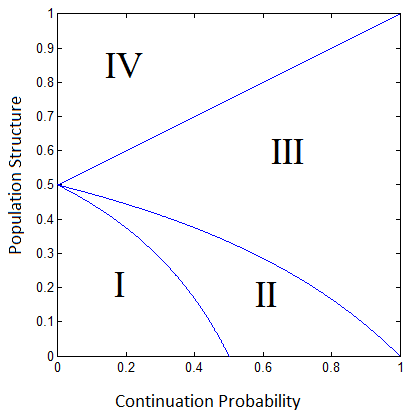
\includegraphics[width=0.7\textwidth]{regions}
\caption{Regions of behaviour for varied continuation probability and structure}
\label{fig:regions}
\end{figure}

In Region I, ALLD is an equilibrium- determined by comparing the payoff of ALLD to a mutant that cooperates at least once. It is not the only equilibrium in the region, but equilibria strategies will play Defect against themselves and ALLD. In this region, cooperation is not expected; no cooperating strategy is an equilibrium.

In Region II, a variety of strategies are equilibria; for example, ALLD and TFT. So, both extremes of behaviour may be seen in a population under these circumstances. 

In Region III, there are again a variety of strategies that are equilibria, but ALLD and other complete defectors are no longer equilibria. Cooperative behaviour of varying types and degrees is expected to be common most of the time (equilibria can be escaped, for a short time).

In Region IV, ALLC is an equilibrium. All other equilibria always cooperate when playing against ALLC or themselves. Fully cooperative behaviour is expected to dominate. More regions are defined, but these are the ones of primary concern.

These general regions are expected to hold regardless of representation (I and II are particularly well defined, and not expected to vary).
The simulations van Veelen et. al. conducted were of FSA with an unbounded number of states and half-memory (of unbounded length). The simulation is initialized with simple individuals: ALLD. Every member plays one other member of the population for a number of rounds determined stochastically, based on the continuation probability. With probability $r$ a member will play against an identical strategy. With probability $1-r$ a member will play against another player from the population. 

This payoff was used to calculate the probability for the individual to reproduce into the next generation. Stochastically, members of the population are selected for the new generation, so unfit individuals tend to be removed. 
During reproduction, mutation could also occur, resulting in new strategies. 

Results of the simulation were consistent with the analysis. 
A colourmap indicating the amount of cooperation in the simulation for varied continuation probabilities and assortment parameters was produced, with behaviour matching that predicted in each region. 
In general, both increased assortment and increased continuation probability increases cooperation (but there are exceptions). 

Indirect invasions are observed in the simulation \citep{garcia:PLoSOne:2012}. 
Indirect invasions are when a new strategy enters the population not by performing well against the currently dominant strategy, but by `springboarding' off another strategy. 
For example, consider that TFT is resistant to ALLD, and will only get exploited on the first move. 
ALLC is a neutral mutant of TFT (it plays against TFT the same way TFT plays against itself), and in a finite population of mostly TFT, ALLC can become more common by neutral drift. 
ALLD can exploit ALLC, and so when this neutral drift occurs, ALLD can use it to invade the population. 
This was summarised as: ``unconditional cooperation is therefore cooperation's worst enemy'' \citep{van-veelen:PNAS:2012}. 
Indirect invasions were observed establishing cooperative behaviour in a defecting population too. 

The results of the analysis should be valid regardless of representation. The simulation built upon previous work, investigating the interplay between reciprocity and population structure, and using unbounded rather than bounded FSAs allowing an infinite strategy space. 
However, the set of all possible strategies for the Prisoner's Dilemma is larger than this space. 

Other representations have their own strategy space. 
The choice of representation will exclude some, and enable some that were not possible in other representations. 
Representation also affects the chance of a strategy appearing, or the route by which it appears, since the mutation process may differ.
 
The model described in \citet{van-veelen:PNAS:2012} was chosen as the basis of my project. 
Both varied assortment and varied chance of a game continuing are modelled. 
Broad behaviour (such as whether strategies that always cooperate can dominate, or can be somewhat successful) can be predicted for ranges of assortment and continuation probability. This provides bounds for what behaviour is expected. 
Detailed behaviour can be discovered through simulation. 
The impact of variations in the simulation- such as changing how strategies are represented- can be compared quantitatively.
By using both assortment and continuation probability, conditions not explored in previous literature (Region III for example in Figure~\ref{fig:regions}) can be investigated.


\section{Expanding the Strategy Space}
\label{sec:stratspace}
Different representations affect the evolution of cooperation - as noted in section~\ref{sec:axelrodEvolving}. 
There are a number of ways to change the representation and allow for a larger strategy space. 
In a lookup table, the number of previous moves a player remembers when making a decision changes the range of strategies that can be represented. 
In a FSA, the maximum number of states limits the strategies that can be represented; however even an unbounded FSA is limited. 
A FSA can determine if a sequence is in a regular language defined by the FSA. 
So, its strategy space is limited to regular strategies. 

Changing the model also allows for different strategies. 
I have focused on simulations with half-memory strategies. 
That is, each agent has access to the history of its opponent's moves. 
The simulation could be changed, and allow each agent access to its own and its opponent's history- it could have full-memory. 
An example of a strategy that can evolve in full-memory simulations but not half-memory simulations is Win-Stay, Lose-Shift. If it successfully cooperates with or exploits the opponent, it continues with the successful strategy. If it loses, for example gets exploited, it tries the other move. 
To accomplish this it of course needs the result; knowing the result \{R,T,S,P\} is equivalent to knowing the history of both players.

\subsection{Representations}
Small strategy spaces can be useful; in Axelrod's original Tournaments \citep{axelrod:Science:1981}, a set of submitted strategies competed, with interesting results. 
A space consisting of 3 strategies- ALLD, ALLC and TFT- was used by \cite{imhof:PNAS:2005} to examine evolutionary cycles when noise is present. 
Useful as small strategy spaces are, it is not certain that the strategies that perform well in a small space will be successful when the strategy space is expanded.

The limitation of FSA representations to regular languages (and further limitation if the number of states is bounded) has been mentioned. 
Does an evolutionarily successful strategy that cannot be represented by an FSA exist (ie. a non-regular strategy)?
I'm not sure, and this is a major aspect I intend to investigate, but a strategy that is very successful at playing the Prisoner's Dilemma in stochastic games (where noise can cause some moves to be performed opposite to what a strategy intended) certainly exists. 
\citet{press2012iterated} described a class of Zero Determinant (ZD) strategies. 
These strategies move so as to set the opponent's score, or to set the ratio between the opponent's score and the ZD player's score. 
The best a strategy can achieve against these is the score or ratio the ZD is attempting to set. 
This is an example of a non-regular strategy that is successful at playing the game against other strategies (ZD are non-regular in general, but regular examples exist; TFT is a ZD strategy). 
This does not mean it would become the most common strategy in an evolutionary environment for a long time. \citet{adami2013evolutionary} showed that coercive ZD strategies will not be stable- it may invade a population, but the advantage of coercion is short-lived. 
 
One extreme example of a representation with a larger strategy space is Turing Machines \citep{Sipser2006}. 
This would include all strategies described by FSA, but additionally all computable strategies. 
Any such simulation would be very complex, and encounter problems such as what to do about machines that never halt.
A suitable `middle-ground' may provide some insight to how the larger strategy space alters the evolution of strategies. One solution would be to move a single step up the Chomsky hierarchy; Push-Down Automata are more powerful than Finite Automata Machines, representing all regular languages plus all context-free languages. 

The size of the strategy space is not the only factor to consider; how that space is explored (via mutations) matters \citep{garcia:PLoSOne:2012}.

\subsection{The Impact of Mutations}
The impact of mutations on how the strategy space might be explored can be demonstrated with a simple lookup table example and a simple FSA example \citep{fogel1993evolving, garcia:PLoSOne:2012}.  
Consider a lookup table of memory 1. It is 3 bits in length- it needs to know what move to perform initially when there is no history (1 bit), and what do do in response to a cooperate or a defect (2 bits). 
ALLD is represented by (111). Suspicious Tit-For-Tat (STFT), which defects initially then reciprocates, is represented by (101). They are one mutation apart- flip the middle bit. 
The simplest FSA representation is a single node, in a non-accept state, with both C and D transitions pointing to itself. The simplest STFT representation is two nodes, an extra transition, and two move transitions (Figure \ref{fig:stft}). Start on a non-accept node, stay on it if the opponent defects, move to an accept node if the opponent cooperates, and so forth. 
The actual distance between ALLD and STFT depends on how the FSA mutations are done- but the mutation distance is longer. 

**** FIGURE ****


\citet{garcia:PLoSOne:2012} explored the impact of differing mutations distances or probabilities (probability of mutating to a particular strategy should be dependent on how many mutations are needed). 
A lookup table to length 3 was used, and games were repeated, without structure. 
In analysing a small set of strategies (such as the 8 in this case), one approach is to assume uniform mutation probabilities. For n strategies, when a mutation occurs it mutates to any individual strategy at the same rate (1/n). So if a uniform mutation model is used, ALLD to STFT has the same probability as ALLD (111) to ALLC (000), which requires 3 bit-flip mutations in a lookup table representation, and ALLD to TFT, which requires 2 bit-flip mutations.

Both simulation and theoretical analysis comparing uniform and bitwise mutations showed that the frequency of cooperative strategies was significantly lower- assumptions made about mutations, or the mutation methods used affect the results of evolutionary simulations. 

It is important to consider these findings for a number of reasons. 
It highlights the need to consider assumptions made when mutating strategies. 
Uniform probability is not a good assumption depending on the model context, how to mutate a FSA or PDA may also be important. For example, a single mutation may be to add a node that connects to itself. 
This might have different results to a single mutation being to add a node, that connects to random other nodes in the Automaton. If mutations are viewed not from a node and transition perspective, but with a representation as a string of bits like in \cite{miller1996coevolution}, mutations could be performed just by flipping bits- a variety of mutation methods are possible, each exploring strategies differently.

Aside from the possibilities for mutations and how they are evaluated (eg. does it resemble something observed in nature? Is it simple?), if there is a difference in results using different representations in simulations, the role the mutation process plays in that difference must be considered. 

\section{Conclusion}
\label{sec:conc}
The various mechanisms for cooperation to evolve that were discussed (Direct Reciprocity and Assortment) have been fairly well explored individually \citep{imhof:PNAS:2005, nowak:Science:2006}. 
When there is sufficient Assortment, the cooperators have the advantage \citep{bergstrom2003algebra}. 
When the game is repeated enough times (with probabilistic length), cooperators have the advantage \citep{Axelrod1984}. 

Developments in research on the evolution of cooperation when these factors are combined has not been explored to the same depth. One aspect that has not been examined is the impact representations with larger strategy spaces will have on the evolution of cooperation.

What are the possible outcomes of expanding the strategy space in a repeated, structured simulation? 
I would expect that the analysis of \citet{van-veelen:PNAS:2012} would hold; the reasoning was not representation-specific. 
Strategies in those regions will follow the predicted behaviour, but the strategies that appear may vary when a different representation is used. 
Recent research, such as \citet{garcia:PLoSOne:2012} indicates the importance of representations and mutations. 
In the case of switching to a Push Down Automata representation, one possibility is that the results are identical. 
PDA have states and transitions like FSA, but add a stack that each transition can access, reading and removing the item at the top of the stack and pushing to the top of the stack. 
A PDA can simulate all FSA, plus additional strategies (Context-Free)\citep{Sipser2006}.  
They are capable of things a FSA is not; for example rudimentary counting with history of any length (eg. push X times to the stack if a Defect is read, pull Y times if Cooperate is read and the stack is not empty. If the stack is empty when all history has been read, Cooperate). If the best strategies inside context-free strategy space are also regular (if those capabilities are not advantageous), it may have the same overall outcomes.  

Another possible outcome is that strategies tend to be more or less cooperative than in the original simulation; that the extra allowed strategies find ways to exploit strategies more, or to establish cooperation more. 
The behaviour within the regions described by \citet{van-veelen:PNAS:2012} may display different patterns; perhaps in one region it tends towards cooperation more than the FSA simulation did, and in another it tends towards defection more. 

We know enough to make some predictions about the behaviour of agents playing the Repeated Prisoner's Dilemma if the representations are changed, so as to allow a larger strategy space. 
We know that no strategy is the best strategy (all strategies can be invaded). 
How the dynamics change when larger strategy spaces are allowed is not fully understood, and is the focus of my research.
\chapter{Contribution Chapters}
\section{Deterministic Pushdown Automata}
%Rambling. Fix.
Non-Deterministic Pushdown Automata have the advantage that they can represent all of the Regular Language strategy space, plus the Context-Free Language strategy space. They have the disadvantage that at any point multiple paths may be followed; a set of valid configurations is needed rather than a single configuration, impacting complexity and runtime. Using Deterministic Pushdown Automata removes this disadvantage, allowing only a single valid configuration. 
It also limits the strategy space; all regular languages are still present, but now it is limited to Deterministic Context-Free Languages; and if only accept by state or only accept by empty stack is allowed, it is further limited. 

A DPDA consists of States which can be accepting or non-accepting, a Stack which contains letters from the Stack Alphabet, a Tape containing letters from the Tape Alphabet which can only be read in one direction, and Transitions. These transitions are followed according when the letter read from the tape matches the Read parameter for that transition, and the stack contains the transitions Pop parameter at the top. As the transition is followed, the State changes to the Destination and the character that is the transitions Push parameter is pushed to the top of the stack. 

The requirements of a DPDA are:



\subsection{Mutation}
As discussed previously *chap ref*, the mutation scheme matters. As long as it is a reasonable exploration of the strategy space we expect certain behaviour to hold, but much of the dynamics will be dependant on the mutation scheme chosen. Since I intend to extend work done with Finite State Automata, I have based my mutation scheme heavily on a mutation scheme for Finite State Automata.

The first mutation is the Add State mutation. A state is generated, which can be either an accepting state or a non-accepting state. Additionally, an outbound transitions is added with random Read, Pop, Push instructions and a random destination (with no bias towards 'nearby' states, or bias against the new state itself as the destination). One transition is rerouted with the new state as its destination, ensuring the new state is connected to the Automaton. 

Alternative mutation schemes could already be noted for just this first mechanism. 
The requirement that the new state be connect could be dropped- perhaps with justification to biologic systems. Inactive, and potentially useless information may exist in a genome. 
It could also be important- at some later stage it may be the subject of an advantageous mutation. 
The connected requirement is made in order to address bloat *a ref here*. 
Another alternative would be to not add any transitions- or to add an inbound transition rather than reroute an existing one. The method chosen is used as it ensures connectedness and is a smaller edit, when we define the size of an edit as the number of parameters changed. Four parameters must be added if a transition is inserted (Read, Pop, Push, Destination), whereas the single re-routing is only one parameter change.

Removing a state is the second method of mutation. Outbound transitions from the state are deleted. 
Inbound states are randomly rerouted. When the re-routing results in an invalid automaton, the transition is deleted instead. Rerouting is chosen over deleting all related transition to minimize the size of the mutation. 

Adding a transition involves randomly selecting a source, destination, and Read Pop and Push instructions. 
\chapter{Discussion Chapters}

\chapter{Conclusion}

\appendix % all \chapter{..} commands after this will generate appendices


\chapter{This appendix should get a letter}
\label{app:example}
An appendix before the backmatter gets an automatically generated letter by
which it can be referred to. This is Appendix~\ref{app:example}.

\chapter{Simulation Source Code}
You may want to investigate the \texttt{lgrind} program and package if you
wish to include source code in your thesis

%%%%%%%%%%%%%%%%%%%%%%%%%%%%%%%%%%%%%%%%%%%%%%%%%%%%%%%%%%%%%%%%%%%%%%%%%%%%%%
%%
%% Back matter 
%%

\backmatter						% start the thesis back matter
\begin{thesisauthorvita}
\begin{spacing}{1}
Publications arising from this thesis include:
\begin{description}
\item[Author, A.\ and Bloggs, J.\ (2002),]
A really catchy title. In \emph{The 31st International Conference
on Non-specific Computing.} Capital City, Country.
\item[Bloggs, J.\ and Author , A. (2002),]
A very much longer and significantly less catchy title. in \emph {Workshop on
A Research Area}. Springfield, USA.
\end{description}
\end{spacing}
\end{thesisauthorvita}

\bibliographystyle{dcu} % A good style to use with the Harvard package
\bibliography{../bibliography}
\chapter{Last Thing} % Appendices after the \backmatter command do not
						% get a letter
This sort of appendix has no letter. 


\end{document}
